\documentclass{article}

\usepackage{fontspec}
\usepackage{fullpage}
\usepackage{multicol}
\usepackage{multirow}
\usepackage{tikz}

\begin{document}

\newfontfamily\swfill{SuttonSignWritingFill.ttf}
\newfontfamily\swline{SuttonSignWritingLine.ttf}
\newcommand{\bul}{\hfil$\bullet$&}
\renewenvironment{glossary}{\begin{multicols}{5}\begin{center}}{\end{center}\end{multicols}}
\setcounter{secnumdepth}{0}
\setlength{\columnseprule}{1pt}

\section{Supplement For Lesson 7}

\begin{center}
\it
Objectives inspired by, vocabulary transcribed from, and sentences and story by Bill Vicars.

Handshape photos by Adam Frost.

No endorsement implied nor given by either.
\end{center}

\subsection{Objectives}

\begin{tabular}{p{1cm}p{14cm}}
\bul I have completed the objectives for this lesson.\\
\bul I understand how dominant hand affects SignWriting.\\
\bul I am able to read the numbers 1,000--999,999.\\
\bul I understand how the ``ABCOS15'' handshapes fit into ASL SignWriting.\\
\bul I am able to demonstrate the meaning and form of the symbol groups in the detail category.\\
\bul I know which base symbols are in Symbol Groups wall and diagonal.\\
\bul I am able to draw the fist heel palmshape in all forms.\\
\bul I am able to draw and demonstrate what fill six means.\\
\bul I am able to read, write, and sign one third of the ASL handshapes in symbol group five.\\
\bul I am able to recognize the vocabulary for this lesson.\\
\bul I am able to read the practice sentences for this lesson.\\
\bul I am able to read the practice story for this lesson.\\
\end{tabular}

\subsection{Dominant Hand and SignWriting}

We covered this long ago back in lesson one.
The full answer is that dominant hand can either have no effect on SignWriting or completely mirror all the handshapes and directions of each word.

If your dominant hand happens to be right, then the sign for clean happens to be B528x522S15a37473x486S15a51482x499S26507515x479S21100500x492 and that is the way we consistently write it.
But the sign for clean is also B517x529S15a3f494x503S15a59493x506S26511484x472S21100498x487 and when reading something written by someone else we must also accept this spelling.
Why?
As you become more comfortable with ASL and SignWriting you will internalize it as being in your voice --- you will process speech/signing as if you are the one speaking/signing.
So if someone has written you a note and it happens to be left hand dominant, that just means that it is how that person thinks.
Normally you might expect a disclaimer along the lines of ``pending teacher approval'' but in this case I'm going to say that if your teacher does not accept it then they are wrong --- it must be acceptable.

Which brings up the question as to why these supplements don't include both spellings?
Primarily it is because of space --- twice as many pages for sample sentences and stories and also the fear about overwhelming the reader.
A secondary reason is that it is well established that right hand dominant is the ``standard'' spelling --- if you find a book in ASL it will be right hand dominant.

So what effect does dominant hand have on SignWriting, usually none.
In cases where it does, here is the effect.

\begin{tabular}{p{1cm}p{14cm}}
\bul Each movement arrow is mirrored.\\
\bul Many movement arrows have their fill changed to reflect the change in handedness.\\
\bul Each hand is mirrored.\\
\bul Each symbol is moved to reverse the horizontal spacing --- vertical spacing remains the same.\\
\bul Noses and other items that we only have one of remain unchanged.\\
\end{tabular}

\subsection{The Numbers 1,000 Through 999,999}

In SignWriting you will almost exclusively be written as a vertical list of the digits for zero through nine.
This is just like English using digits to write out large numbers.
This lesson will, in contrast to normal usage, be showing the full words --- instead of 1,234 you will see one thousand two hundred thirty four.
Just like in English, writing the full words takes more space but given the goal of this supplement it is required.

In future lessons we will eventually switch to using digits, as you would normally see in SignWriting, but you must remember to interpret the digits and use the correct signs when speaking in ASL.

\begin{center}
\begin{tabular}{*{5}{c}}
\textbf{1,000}&\textbf{2,000}&\textbf{3,000}&\textbf{4,000}&\textbf{5,000}\\
B521x540S20500479x525S15a38492x513S18051496x515S10020502x461S22a04503x495&
B521x540S20500479x525S15a38492x513S18051496x515S10e20501x461S22a04503x495&
B521x540S20500479x525S15a38492x513S18051496x515S22a04503x495S11e20494x461&
B522x540S20500479x525S15a38492x513S18051496x515S22a04503x495S14420500x461&
B521x540S20500479x525S15a38492x513S18051496x515S22a04503x495S14c20498x461\\
\textbf{6,000}&\textbf{7,000}&\textbf{8,000}&\textbf{9,000}\\
B521x540S20500479x525S15a38492x513S18051496x515S22a04503x495S18720500x461&
B522x539S20500479x524S15a38492x512S18051496x514S22a04503x494S1a520501x462&
B522x539S20500479x524S15a38492x512S18051496x514S22a04503x494S1bb20501x462&
B523x540S20500478x525S15a38491x513S18051495x515S22a04502x495S1ce20501x461\\
\end{tabular}
\end{center}

\subsection{The ``ABCOS15'' Handshapes and ASL SignWriting}

The simple takeaway from ``ABCOS15'' is that SignWriting has B510x508S1f708490x493, B506x514S15a08494x487, B509x510S16d08492x490, B508x508S17600492x492, B508x508S20308493x493, B508x515S10008493x485, and B512x516S14c08489x485;
but there is so much more to consider.

English, at least American English, now has words and phrases which were originally borrowed from other languages like \textsc{rsvp}, je ne sais quoi, adios, lariat.
As these words and phrases become more anglicized, the pronunciation and even the meaning adjusted.
\textsc{Rsvp} is a literal request for a response regardless of the response, but for most speakers of American English it means respond but only if you are coming.
\emph{La reata} literally means ``the rope'' but was merged into a single word, had the last syllable dropped, and the stress moved forward, as well as becoming a special form of its original meaning.

English is not the only language to do these types of things.
In fact, this is so common it would be rather strange for ASL to \emph{not} do this.
The difference is that while ASL \emph{can} borrow from other sign languages, it is \emph{more likely} to borrow from English spelling and/or pantomiming in spaces not occupied by current words.
This is how we start with and still have initialized words in ASL as well as words that are visually descriptive, but as native speakers become more comfortable with the concept and make it their own the handshapes will move from ``well formed letters'' into some basic handshapes which, movements, and locations.
That is, words that start with B508x515S11500493x485 or B510x513S18d00490x488, are likely to become B512x508S18200489x493 over time;
many words that start with both hands moving are likely to simplify to either a dominant hand moving while the non-dominant hand remains stationary or both hands making the same movement;
and words that start around the waist are likely to move up over time.

For the dominant hand, the number of handshapes available is rather larger --- these lessons cover what has been identified as the basic handshapes for the dominant hand and it's just over eighty.
For the non-dominant hand, these handshapes are likely to simplify to this much smaller set of about seven shapes both because these are the standard shapes and because native speakers learning new words aren't interested in the exact shape as they learn to speak but in maintaining correct understanding.

\subsection{The Detail Category}

We informally call this category detail, though it's official name is ``Detailed Location'' and it has one base symbol in it with the same name.

\begin{center}
\begin{tabular}{ccc}
\textbf{Symbol}\\
\textbf{Group}&\textbf{Name}&\textbf{Example}\\
\textbf{29}&Detail&B521x521S37f00480x480\\
\end{tabular}
\end{center}

\subsection{The Symbol Groups Wall and Diagonal}

The thirteenth Symbol Group we informally call wall, though it's official name is ``Straight Wall Plane''.
Symbol Group Straight Wall Plane (Wall) has all types of vertical movement --- up and down though left and right movement can also be shown.
Each of these arrows have a pair of tails, to remind us of a rocket ship blasting off vertically.

\begin{center}
\begin{tabular}{rcrc}
\textbf{Base Symbol}&\textbf{Example}&\textbf{Base Symbol}&\textbf{Example}\\
Single Straight Movement, Wall Plane Small&B507x508S22a00494x493&Single Straight Movement, Wall Plane Medium &B508x515S22b00492x485\\
Single Straight Movement, Wall Plane Large&B508x521S22c00492x479&Single Straight Movement, Wall Plane Largest&B508x525S22d00492x475\\
Single Wrist Flex, Wall Plane             &B509x509S22e00492x491&Double Straight Movement, Wall Plane        &B513x507S22f00488x493\\
Double Wrist Flex, Wall Plane             &B513x509S23000488x491&Double Alternating Movement, Wall Plane     &B513x509S23100487x492\\
Double Alternating Wrist Flex, Wall Plane &B513x510S23200487x490&Cross Movement, Wall Plane                  &B515x513S23300485x487\\
Triple Straight Movement, Wall Plane      &B519x507S23400482x493&Triple Wrist Flex, Wall Plane               &B519x509S23500482x491\\
Triple Alternating Movement, Wall Plane   &B520x509S23600481x492&Triple Alternating Wrist Flex, Wall Plane   &B520x511S23700481x490\\
Bend, Wall Plane Small                    &B509x513S23800492x488&Bend, Wall Plane Medium                     &B510x515S23900490x485\\
Bend, Wall Plane Large                    &B513x521S23a00487x479&Corner, Wall Plane Small                    &B510x511S23b00491x490\\
Corner, Wall Plane Medium                 &B512x514S23c00489x487&Corner, Wall Plane Large                    &B514x517S23d00487x483\\
Corner, Wall Plane with Rotation          &B515x516S23e00485x484&Check, Wall Plane Small                     &B511x514S23f00490x486\\
Check, Wall Plane Medium                  &B513x517S24000487x483&Check, Wall Plane Large                     &B514x520S24100486x481\\
Box, Wall Plane Small                     &B512x511S24200488x489&Box, Wall Plane Medium                      &B515x514S24300486x487\\
Box, Wall Plane Large                     &B517x517S24400484x484&Zigzag, Wall Plane Small                    &B509x516S24500491x485\\
Zigzag, Wall Plane Medium                 &B512x520S24600488x481&Zigzag, Wall Plane Large                    &B513x522S24700487x479\\
Peaks, Wall Plane Small                   &B508x514S24800492x486&Peaks, Wall Plane Medium                    &B510x518S24900491x482\\
Peaks, Wall Plane Large                   &B511x524S24a00490x477&Travel Rotation, Single Wall Plane          &B511x513S24b00489x487\\
Travel Rotation, Double Wall Plane        &B511x518S24c00489x483&Travel Rotation, Alternating Wall Plane     &B512x518S24d00488x483\\
Travel Rotation, Single Floor Plane       &B511x515S24e00490x485&Travel Rotation, Double Floor Plane         &B510x518S24f00490x482\\
Travel Rotation, Alternating Floor Plane  &B511x518S25000489x482&Travel Shaking, Wall Plane                  &B509x517S25100491x484\\
Travel Arm Spiral, Wall Plane Single      &B513x518S25200488x483&Travel Arm Spiral, Wall Plane Double        &B513x521S25300488x479\\
Travel Arm Spiral, Wall Plane Triple      &B513x525S25400488x475\\
\end{tabular}
\end{center}

The fourteenth Symbol Group we informally call diagonal, though it's official name is ``Straight Diagonal Movement''.
Symbol Group Straight Diagonal Movement (Diagonal) has all ways the movement that is both horizontal and vertical at the same time.
It is shown to be primarily vertical but the movement away from you will have an extra line --- like looking at the tail of a jet moving away from you.
Movement towards you will have an extra circle --- like watching the nose of a jet coming straight at you.

\begin{center}
\begin{tabular}{rcrc}
\textbf{Base Symbol}&\textbf{Example}&\textbf{Base Symbol}&\textbf{Example}\\
Diagonal Away Movement Small   &B507x511S25500494x489&Diagonal Away Movement Medium    &B508x515S25600492x485\\
Diagonal Away Movement Large   &B508x521S25700492x479&Diagonal Away Movement Largest   &B508x525S25800492x475\\
Diagonal Towards Movement Small&B507x512S25900493x489&Diagonal Towards Movement Medium &B508x515S25a00492x485\\
Diagonal Towards Movement Large&B508x521S25b00492x479&Diagonal Towards Movement Largest&B508x525S25c00492x475\\
Diagonal Between Away Small    &B507x510S25d00493x490&Diagonal Between Away Medium     &B508x515S25e00492x485\\
Diagonal Between Away Large    &B508x520S25f00492x480&Diagonal Between Away Largest    &B508x525S26000492x475\\
Diagonal Between Towards Small &B507x510S26100493x491&Diagonal Between Towards Medium  &B508x515S26200492x485\\
Diagonal Between Towards Large &B508x521S26300492x479&Diagonal Between Towards Largest &B508x525S26400492x475\\
\end{tabular}
\end{center}

Before you can consider this lesson complete, you need to be able to list off the symbol groups as:
``one, two, three, four, five, six, seven, eight, nine, thumb;''
``contact, finger, wall, diagonal.''

Some additional help when remembering the second set of base symbols.
Contact and finger you will just have to remember, but now point to the wall and rotate your arm till your index finger points down to the floor.

This is the order followed by the base symbols in the second set --- wall first, floor last.
You can consider this lesson complete when you can remember ``contact, finger, wall, diagonal,'' but you should be able to guess that the next symbol is floor because ``wall first, floor last.''

\subsection{The Fist Heel Palmshape}

The Fist Heel Palmshape only comes as fill 2 which in the case of the primary rotation means palm up.
The idea is that when you are focused on the heel, you can see both the palm and the back of the hand at the same time so fills 1, 3, 4, and 6 cannot occur.
The reason fill 5 is missing is because of the physiology of human arms --- you won't be using the heel handshape with palm towards the signer.

\begin{center}
\begin{tabular}{r*{6}{c}}
&\textbf{Fill 1}&\textbf{Fill 2}&\textbf{Fill 3}&\textbf{Fill 4}&\textbf{Fill 5}&\textbf{Fill 6}\\
\textbf{Right}&---&B508x506S20410493x495&---&---&---&---\\
\textbf{Left} &---&B508x506S20418493x495&---&---&---&---\\
\end{tabular}
\end{center}

\subsection{The Sixth Fill}

\subsubsection{Hand Symbols}

\begin{center}
B508x515S10050493x485 B508x515S10e50493x485 B512x515S11e50489x485
\end{center}

Any handshape symbol drawn in the sixth fill means that the signer's palm is facing down.
For all the hand symbols, the empty portion represents the signer's palm and the filled portion represents the back of the hand.
So for fill six the palm is completely filled in.

\subsubsection{Everything Else}

\begin{center}
B518x518S30a50482x483
\end{center}

The fills for other categories tend to be a bit more variable.
Here we have the left eyebrow raised by itself.

\subsection{First ASL Handshapes From Symbol Group Five}

The twenty one handshapes in Symbol Group Five used by ASL in order are:
{\it
Five Fingers Spread;
Five Fingers Spread Heel;
Five Fingers Spread, Four Bent;
Five Fingers Spread, Four Bent Heel;
Five Fingers Spread Bent;
Five Fingers Spread Bent Heel;
Five Fingers Spread Cup;
}
Five Fingers Spread Cup Open;
Five Fingers Spread Hinge;
Flat Hand;
Flat Heel;
Flat, Thumb Side;
Flat, Thumb Side Heel;
Cup;
Cup, Thumb Side;
Cup, No Thumb;
Circle;
Hinge;
Hinge, Thumb Side
Hinge, No Thumb
and Angle.

\subsubsection{The Five Fingers Spread Handshape}

\begin{center}
\begin{tabular}{r*{6}{c}}
&\textbf{Fill 1}&\textbf{Fill 2}&\textbf{Fill 3}&\textbf{Fill 4}&\textbf{Fill 5}&\textbf{Fill 6}\\
\multirow{2}{*}{\textbf{Right}}&
B512x516S14c00489x485&
B512x516S14c10489x485&
B512x516S14c20489x485&
B512x516S14c30489x485&
B512x516S14c40489x485&
B512x516S14c50489x485\\
&
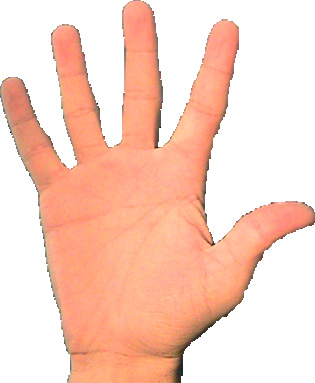
\includegraphics[scale=0.1]{images/05-01-1.jpg}&
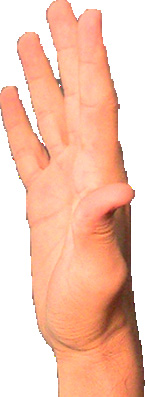
\includegraphics[scale=0.1]{images/05-01-2.jpg}&
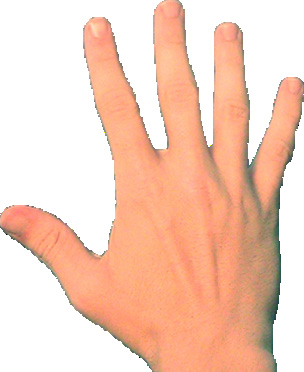
\includegraphics[scale=0.1]{images/05-01-3.jpg}&
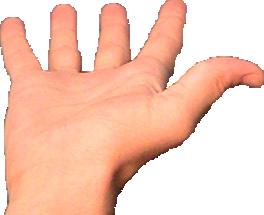
\includegraphics[scale=0.1]{images/05-01-4.jpg}&
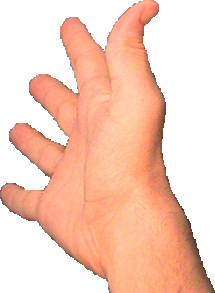
\includegraphics[scale=0.1]{images/05-01-5.jpg}&
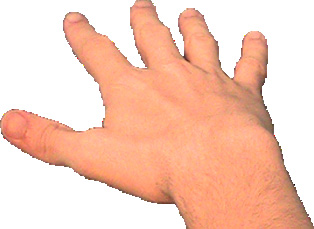
\includegraphics[scale=0.1]{images/05-01-6.jpg}\\
\textbf{Left}&
B512x516S14c08489x485&
B512x516S14c18489x485&
B512x516S14c28489x485&
B512x516S14c38489x485&
B512x516S14c48489x485&
B512x516S14c58489x485\\
\end{tabular}
\end{center}

\subsubsection{The Five Fingers Spread Heel Handshape}

\begin{center}
\begin{tabular}{r*{6}{c}}
&\textbf{Fill 1}&\textbf{Fill 2}&\textbf{Fill 3}&\textbf{Fill 4}&\textbf{Fill 5}&\textbf{Fill 6}\\
\multirow{2}{*}{\textbf{Right}}&
\multirow{2}{*}{---}&
B515x509S14d10485x491&
\multirow{2}{*}{---}&
\multirow{2}{*}{---}&
\multirow{2}{*}{---}&
\multirow{2}{*}{---}\\
&
&
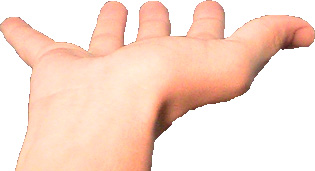
\includegraphics[scale=0.1]{images/05-02-2.jpg}\\
\textbf{Left}&
---&
B515x509S14d18485x491&
---&
---&
---&
---\\
\end{tabular}
\end{center}

\subsubsection{The Five Fingers Spread, Four Bent Handshape}

\begin{center}
\begin{tabular}{r*{6}{c}}
&\textbf{Fill 1}&\textbf{Fill 2}&\textbf{Fill 3}&\textbf{Fill 4}&\textbf{Fill 5}&\textbf{Fill 6}\\
\multirow{2}{*}{\textbf{Right}}&
B513x516S14e00488x485&
B513x516S14e10488x485&
B513x516S14e20488x485&
B513x516S14e30488x485&
B513x516S14e40488x485&
B513x516S14e50488x485\\
&
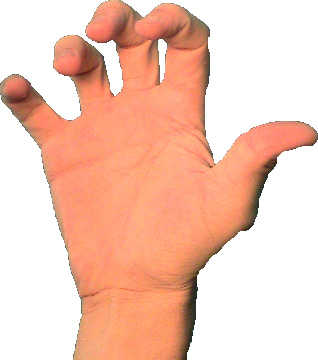
\includegraphics[scale=0.1]{images/05-03-1.jpg}&
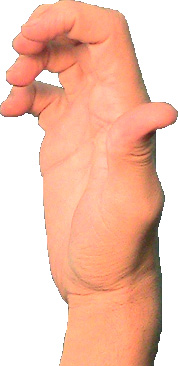
\includegraphics[scale=0.1]{images/05-03-2.jpg}&
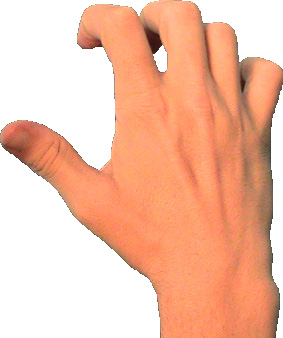
\includegraphics[scale=0.1]{images/05-03-3.jpg}&
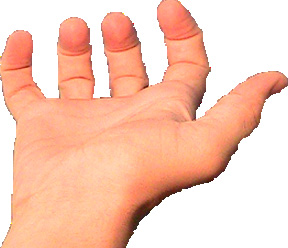
\includegraphics[scale=0.1]{images/05-03-4.jpg}&
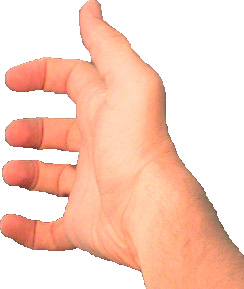
\includegraphics[scale=0.1]{images/05-03-5.jpg}&
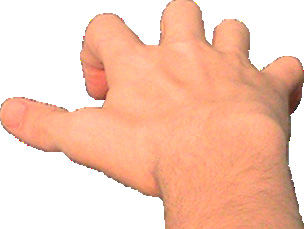
\includegraphics[scale=0.1]{images/05-03-6.jpg}\\
\textbf{Left}&
B513x516S14e08488x485&
B513x516S14e18488x485&
B513x516S14e28488x485&
B513x516S14e38488x485&
B513x516S14e48488x485&
B513x516S14e58488x485\\
\end{tabular}
\end{center}

\subsubsection{The Five Fingers Spread, Four Bent Heel Handshape}

\begin{center}
\begin{tabular}{r*{6}{c}}
&\textbf{Fill 1}&\textbf{Fill 2}&\textbf{Fill 3}&\textbf{Fill 4}&\textbf{Fill 5}&\textbf{Fill 6}\\
\multirow{2}{*}{\textbf{Right}}&
\multirow{2}{*}{---}&
B515x508S14f10485x492&
\multirow{2}{*}{---}&
\multirow{2}{*}{---}&
\multirow{2}{*}{---}&
\multirow{2}{*}{---}\\
&
&
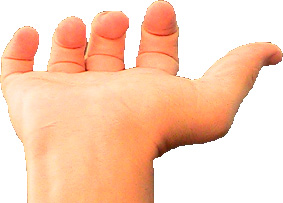
\includegraphics[scale=0.1]{images/05-04-2.jpg}\\
\textbf{Left}&
---&
B515x508S14f18485x492&
---&
---&
---&
---\\
\end{tabular}
\end{center}

\subsubsection{The Five Fingers Spread Bent Handshape}

\begin{center}
\begin{tabular}{r*{6}{c}}
&\textbf{Fill 1}&\textbf{Fill 2}&\textbf{Fill 3}&\textbf{Fill 4}&\textbf{Fill 5}&\textbf{Fill 6}\\
\multirow{2}{*}{\textbf{Right}}&
B513x516S15000488x485&
B513x516S15010488x485&
B513x516S15020488x485&
B513x516S15030488x485&
B513x516S15040488x485&
B513x516S15050488x485\\
&
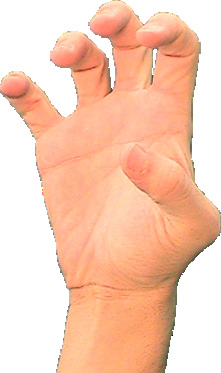
\includegraphics[scale=0.1]{images/05-05-1.jpg}&
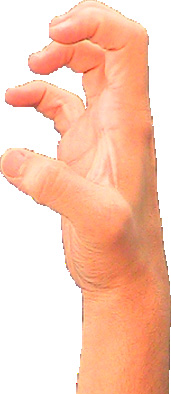
\includegraphics[scale=0.1]{images/05-05-2.jpg}&
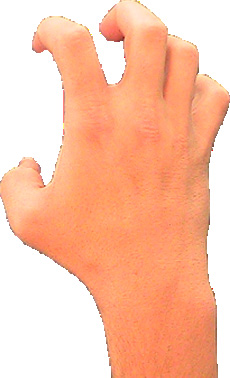
\includegraphics[scale=0.1]{images/05-05-3.jpg}&
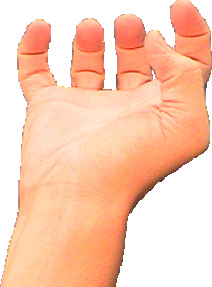
\includegraphics[scale=0.1]{images/05-05-4.jpg}&
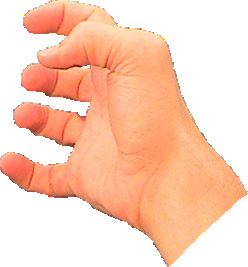
\includegraphics[scale=0.1]{images/05-05-5.jpg}&
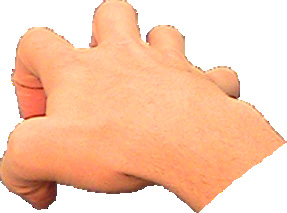
\includegraphics[scale=0.1]{images/05-05-6.jpg}\\
\textbf{Left}&
B513x516S15008488x485&
B513x516S15018488x485&
B513x516S15028488x485&
B513x516S15038488x485&
B513x516S15048488x485&
B513x516S15058488x485\\
\end{tabular}
\end{center}

\subsubsection{The Five Fingers Spread Bent Heel Handshape}

\begin{center}
\begin{tabular}{r*{6}{c}}
&\textbf{Fill 1}&\textbf{Fill 2}&\textbf{Fill 3}&\textbf{Fill 4}&\textbf{Fill 5}&\textbf{Fill 6}\\
\multirow{2}{*}{\textbf{Right}}&
\multirow{2}{*}{---}&
B515x508S15110486x492&
\multirow{2}{*}{---}&
\multirow{2}{*}{---}&
\multirow{2}{*}{---}&
\multirow{2}{*}{---}\\
&
&
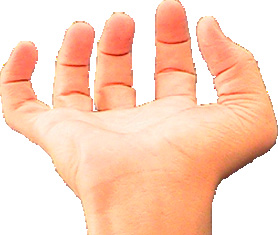
\includegraphics[scale=0.1]{images/05-06-2.jpg}\\
\textbf{Left}&
---&
B515x508S15118486x492&
---&
---&
---&
---\\
\end{tabular}
\end{center}

\subsubsection{The Five Fingers Spread Cup Handshape}

\begin{center}
\begin{tabular}{r*{6}{c}}
&\textbf{Fill 1}&\textbf{Fill 2}&\textbf{Fill 3}&\textbf{Fill 4}&\textbf{Fill 5}&\textbf{Fill 6}\\
\multirow{2}{*}{\textbf{Right}}&
B508x513S15300493x488&
B508x513S15310493x488&
B508x513S15320493x488&
B508x513S15330493x488&
B508x513S15340493x488&
B508x513S15350493x488\\
&
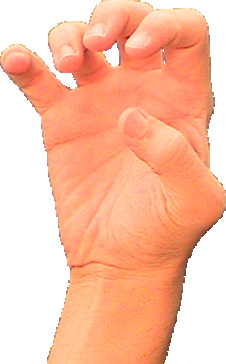
\includegraphics[scale=0.1]{images/05-07-1.jpg}&
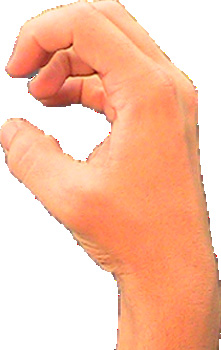
\includegraphics[scale=0.1]{images/05-07-2.jpg}&
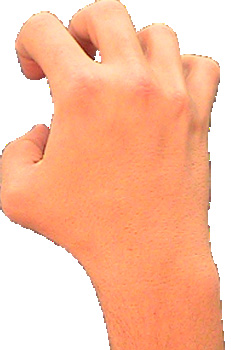
\includegraphics[scale=0.1]{images/05-07-3.jpg}&
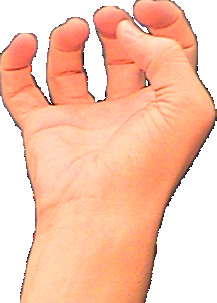
\includegraphics[scale=0.1]{images/05-07-4.jpg}&
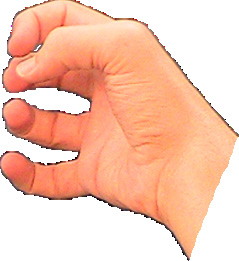
\includegraphics[scale=0.1]{images/05-07-5.jpg}&
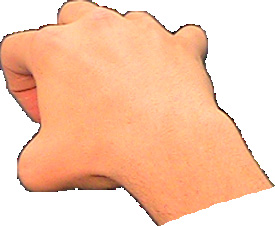
\includegraphics[scale=0.1]{images/05-07-6.jpg}\\
\textbf{Left}&
B508x513S15308493x488&
B508x513S15318493x488&
B508x513S15328493x488&
B508x513S15338493x488&
B508x513S15348493x488&
B508x513S15358493x488\\
\end{tabular}
\end{center}

\subsection{Vocabulary}

\begin{glossary}

\textbf{1,000}\\
AS10020S22a04S18051S15a38S20500M521x540S20500479x525S15a38492x513S18051496x515S10020502x461S22a04503x495

\textbf{2,000}\\
AS10e20S22a04S18051S15a38S20500M521x540S20500479x525S15a38492x513S18051496x515S10e20501x461S22a04503x495

\textbf{3,000}\\
AS11e20S22a04S18051S15a38S20500M521x540S20500479x525S15a38492x513S18051496x515S22a04503x495S11e20494x461

\textbf{4,000}\\
AS14420S22a04S18051S15a38S20500M522x540S20500479x525S15a38492x513S18051496x515S22a04503x495S14420500x461

\textbf{5,000}\\
AS14c20S22a04S18051S15a38S20500M521x540S20500479x525S15a38492x513S18051496x515S22a04503x495S14c20498x461

\textbf{6,000}\\
AS18720S22a04S20500S18051S15a38M521x540S20500479x525S15a38492x513S18051496x515S22a04503x495S18720500x461

\textbf{7,000}\\
AS1a520S22a04S18051S15a38S20500M522x539S20500479x524S15a38492x512S18051496x514S22a04503x494S1a520501x462

\textbf{8,000}\\
AS1bb20S22a04S18051S15a38S20500M522x539S20500479x524S15a38492x512S18051496x514S22a04503x494S1bb20501x462

\textbf{9,000}\\
AS1ce20S22a04S18051S15a38S20500M523x540S20500478x525S15a38491x513S18051495x515S22a04502x495S1ce20501x461

\textbf{and}\\
AS14c02S26506S18500M543x512S14c02458x489S26506496x492S18500519x494

\textbf{apple}\\
AS10612S2c400S2ff00M563x526S2ff00482x483S10612515x511S2c400523x483

\textbf{bologna}\\
AS17650S17658S22a06S22a22S2fb00S20350S20358M560x513S17650482x487S17654507x487S20350545x488S20350440x487S22a06526x489S22a12460x488S2fb04495x507

\textbf{candy}\\
AS10011S2e000S20500S2ff00M541x542S2ff00482x483S10011510x512S20500504x518S2e000520x485

\textbf{cereal}\\
AS10612S22a02S21800S2ff00M518x552S2ff00482x483S10612484x520S21800462x522S22a02494x539

\textbf{cheese}\\
AS14c20S14c0aS21100S2a400M524x546S2a400483x455S14c20484x500S14c0a493x522S21100477x532

\textbf{cookie}\\
AS15051S15a3aS20500S2df08S20500M523x537S15a3a490x494S20500482x481S20500513x481S2df08491x464S15051477x509

\textbf{cup}\\
AS16d40S22f04S15d39S20600M513x543S16d40492x457S22f04488x483S20600489x506S15d39487x520

\textbf{drink}\\
AS16d10S2d201S33b00M518x567S33b00482x483S16d10492x520S2d201490x544

\textbf{eat}\\
AS18507S20500S33b00M528x537S33b00482x483S18507502x510S20500518x509

\textbf{egg}\\
AS11501S11509S28905S2891dS20500S2fb04M540x541S20500496x459S11501506x479S11509471x479S28905513x516S2891d460x515S2fb04493x523

\textbf{food}\\
AS18507S20600S33b00M540x537S33b00482x483S18507502x510S20600518x509

\textbf{full}\\
AS15a51S20348S26603S20e00M529x519S15a51506x482S20348492x504S20e00489x489S26603472x481

\textbf{full}\\
AS14712S22b00S2ff00M518x570S2ff00482x483S14712488x519S22b00493x540

\textbf{hamburger}\\
AS16d21S17107S20800S16d29S1710fS20800M515x543S20800505x533S20800486x457S16d21488x471S1710f490x507S17107496x466S16d29492x513

\textbf{hotdog}\\
AS17650S17658S22a06S22a22S2fb00S20350S20358M560x513S17650482x487S17654507x487S20350545x488S20350440x487S22a06526x489S22a12460x488S2fb04495x507

\textbf{hungry}\\
AS15402S21100S22c04M513x542S15402488x458S21100493x478S22c04490x500

\textbf{kind (an in type)}\\
AS14240S14249S2e800S20500M524x532S14249491x508S14240477x480S2e800510x469S20500480x509

\textbf{milk}\\
AS16d40S21802M515x511S21802485x493S16d40497x490

\textbf{pizza}\\
AS11820S2470aS1f720M550x522S1f720530x506S11820451x478S2470a482x496

\textbf{popcorn}\\
AS1eb07S1eb0fS21d00S21d00S2eb00S2eb48S2fd04M524x546S1eb07504x465S1eb0f476x476S2eb48480x508S21d00478x465S2eb00507x499S21d00500x454S2fd04497x540

\textbf{sausage}\\
AS17650S17658S22a06S22a22S2fb00S20350S20358M560x513S17650482x487S17654507x487S20350545x488S20350440x487S22a06526x489S22a12460x488S2fb04495x507

\textbf{soup}\\
AS11502S15d09S2ea00S20f00M518x585S15d09463x556S11502481x570S2ea00494x521S20f00489x551S33b00482x483

\textbf{style}\\
AS14240S14249S2e800S20500M524x532S14249491x508S14240477x480S2e800510x469S20500480x509

\textbf{taste}\\
AS1c50fS20500S33b00M518x539S1c50f476x514S33b00482x483S20500500x519

\textbf{thousand}\\
AS18051S15a38S20500M521x514S20500479x499S15a38492x487S18051496x489

\textbf{type}
AS14240S14249S2e800S20500M524x532S14249491x508S14240477x480S2e800510x469S20500480x509

\textbf{water}\\
AS18610S20600S2ff00M534x549S20600512x513S2ff00482x483S18610492x519

\textbf{wish}\\
AS15402S21100S22c04M513x542S15402488x458S21100493x478S22c04490x500

\end{glossary}

\subsection{Practice Sheet 7.A}

\begin{multicols}{5}
\begin{center}

M508x515S10000493x485 % 1
\\M536x504S38800464x496 % .
\\M563x526S2ff00482x483S10612515x511S2c400523x483 % apple
\\M537x504S38700463x496 % ,
\\M516x526S1f000484x474S2e230497x494 % green
\\M537x504S38700463x496 % ,
\\M518x518S30a00482x483 % y/n
\\M510x523S10040495x493S26500491x478 % you
\\M516x540S1bb02488x461S14c02484x517S20e00499x502S26500499x483 % like
\\M528x537S33b00482x483S18507502x510S20500518x509 % eat
\\M536x507S38900464x493 % ?
\vfil
\columnbreak

M508x515S10e00493x485 % 2
\\M536x504S38800464x496 % .
\\M541x542S2ff00482x483S10011510x512S20500504x518S2e000520x485 % candy
\\M537x504S38700463x496 % ,
\\M510x523S10040495x493S26500491x478 % you
\\M516x540S1bb02488x461S14c02484x517S20e00499x502S26500499x483 % like
\\M518x518S30c00482x483 % \?
\\M524x532S14249491x508S14240477x480S2e800510x469S20500480x509 % kind
\\M536x507S38900464x493 % ?
\vfil
\columnbreak

M512x515S11e00489x485 % 3
\\M536x504S38800464x496 % .
\\M518x552S2ff00482x483S10612484x520S21800462x522S22a02494x539 % cereal
\\M537x504S38700463x496 % ,
\\M510x523S10040495x493S26500491x478 % you
\\M516x540S1bb02488x461S14c02484x517S20e00499x502S26500499x483 % like
\\M518x518S30c00482x483 % \?
\\M524x532S14249491x508S14240477x480S2e800510x469S20500480x509 % kind
\\M536x507S38900464x493 % ?
\vfil
\columnbreak

M511x516S14400489x485 % 4
\\M536x504S38800464x496 % .
\\M518x518S30a00482x483 % y/n
\\M510x523S10040495x493S26500491x478 % you
\\M516x540S1bb02488x461S14c02484x517S20e00499x502S26500499x483 % like
\\M523x537S15a3a490x494S20500482x481S20500513x481S2df08491x464S15051477x509 % cookie
\\M521x515S1f748479x500S1f740501x500S20500495x485 % with
\\M515x511S21802485x493S16d40497x490 % milk
\\M536x507S38900464x493 % ?
\vfil
\columnbreak

M512x516S14c00489x485 % 5
\\M536x504S38800464x496 % .
\\M534x549S20600512x513S2ff00482x483S18610492x519 % water
\\M510x523S10040495x493S26500491x478 % you
\\M518x567S33b00482x483S16d10492x520S2d201490x544 % drink
\\M541x520S26a00514x474S2ff00482x483S20e00521x490S1f710514x505 % daily
\\M537x504S38700463x496 % ,
\\M513x543S16d40492x457S22f04488x483S20600489x506S15d39487x520 % cup
\\M526x535S22a20494x501S14c08474x465S14c00503x465S20338478x520S20330508x520 % how many
\\M510x523S10040495x493S26500491x478 % you
\\M536x507S38900464x493 % ?
\vfil

\end{center}
\end{multicols}

\subsection{Practice Sheet 7.B}

\begin{multicols}{5}
\begin{center}

M509x515S18720491x486 % 6
\\M536x504S38800464x496 % .
\\M518x518S30c00482x483 % \?
\\M507x523S15a28494x496S26500493x477 % your
\\M540x543S1c507499x518S20600518x508S2ff00482x483 % favorite
\\M540x537S33b00482x483S18507502x510S20600518x509 % food
\\M553x518S2fb04492x512S26c0a538x483S26c12448x488S14c39468x483S14c31506x483 % what
\\M536x507S38900464x493 % ?
\vfil
\columnbreak

M511x514S1a520490x486 % 7
\\M536x504S38800464x496 % .
\\M516x526S1f000484x474S2e230497x494 % green
\\M540x541S20500496x459S11501506x479S11509471x479S28905513x516S2891d460x515S2fb04493x523 % egg
\\M543x512S14c02458x489S26506496x492S18500519x494 % and
\\M515x508S11502485x493 % h
\\M510x508S1f720490x493 % a
\\M510x513S18d20490x488 % m
\\M510x523S10040495x493S26500491x478 % you
\\M516x540S1bb02488x461S14c02484x517S20e00499x502S26500499x483 % like
\\M518x518S30a00482x483 % y/n
\\M510x523S10040495x493S26500491x478 % you
\\M536x507S38900464x493 % ?
\vfil
\columnbreak

M511x514S1bb20490x486 % 8
\\M536x504S38800464x496 % .
\\M518x553S21600497x545S16d10492x520S33b00482x483 % orange
\\M537x504S38700463x496 % ,
\\M518x518S30a00482x483 % y/n
\\M510x523S10040495x493S26500491x478 % you
\\M516x540S1bb02488x461S14c02484x517S20e00499x502S26500499x483 % like
\\M528x537S33b00482x483S18507502x510S20500518x509 % eat
\\M536x507S38900464x493 % ?
\vfil
\columnbreak

M511x515S1ce20489x485 % 9
\\M536x504S38800464x496 % .
\\M518x518S30a00482x483 % y/n
\\M510x523S10040495x493S26500491x478 % you
\\M518x570S2ff00482x483S14712488x519S22b00493x540 % full (under chin)
\\M536x507S38900464x493 % ?
\vfil
\columnbreak

M513x528S2a538494x472S1f540488x504 % 10
\\M536x504S38800464x496 % .
\\M518x518S30c00482x483 % \?
\\M510x523S10040495x493S26500491x478 % you
\\M540x543S1c507499x518S20600518x508S2ff00482x483 % favorite
\\M537x504S38700463x496 % ,
\\R515x543S20800505x533S20800486x457S16d21488x471S1710f490x507S17107496x466S16d29492x513 % hamburger
\\L560x513S17650482x487S17654507x487S20350545x488S20350440x487S22a06526x489S22a12460x488S2fb04495x507 % hotdog
\\M536x507S38900464x493 % ?
\vfil

\end{center}
\end{multicols}

\subsection{Practice Sheet 7.C}

\begin{multicols}{5}
\begin{center}

M512x520S10000489x490S21d00494x480 % 11
\\M536x504S38800464x496 % .
\\M518x518S30c00482x483 % \?
\\M513x542S15402488x458S21100493x478S22c04490x500 % hungry
\\M510x523S10040495x493S26500491x478 % you
\\M536x507S38900464x493 % ?
\vfil
\columnbreak

M509x521S10e00491x491S21d00491x480 % 12
\\M536x504S38800464x496 % .
\\M550x522S1f720530x506S11820451x478S2470a482x496 % pizza
\\M537x504S38700463x496 % ,
\\M518x518S30c00482x483 % \?
\\M510x523S10040495x493S26500491x478 % you
\\M516x540S1bb02488x461S14c02484x517S20e00499x502S26500499x483 % like
\\M524x532S14249491x508S14240477x480S2e800510x469S20500480x509 % kind
\\M536x507S38900464x493 % ?
\vfil
\columnbreak

M513x519S22114487x481S12d00489x489 % 13
\\M536x504S38800464x496 % .
\\M563x518S2ff00482x483S19200542x478S26a04519x487S20500504x501 % suppose
\\M510x523S10040495x493S26500491x478 % you
\\M525x526S10018476x477S10018497x496S2882a503x475 % go
\\M542x523S10058459x493S14c10482x477S20500476x501S2a502509x490 % movie
\\M537x504S38700463x496 % ,
\\M518x518S30a00482x483 % y/n
\\M510x523S10040495x493S26500491x478 % you
\\M516x540S1bb02488x461S14c02484x517S20e00499x502S26500499x483 % like
\\M528x537S33b00482x483S18507502x510S20500518x509 % eat
\\M524x546S1eb07504x465S1eb0f476x476S2eb48480x508S21d00478x465S2eb00507x499S21d00500x454S2fd04497x540 % popcorn
\\M536x507S38900464x493 % ?
\vfil
\columnbreak

M513x515S14700493x493S22114487x486 % 14
\\M536x504S38800464x496 % .
\\M518x585S15d09463x556S11502481x570S2ea00494x521S20f00489x551S33b00482x483 % soup
\\M537x504S38700463x496 % ,
\\M518x518S30c00482x483 % \?
\\M510x523S10040495x493S26500491x478 % you
\\M516x540S1bb02488x461S14c02484x517S20e00499x502S26500499x483 % like
\\M524x532S14249491x508S14240477x480S2e800510x469S20500480x509 % kind
\\M536x507S38900464x493 % ?
\vfil
\columnbreak

M513x518S22114487x483S15d00494x491 % 15
\\M536x504S38800464x496 % .
\\M563x526S2ff00482x483S10612515x511S2c400523x483 % apple
\\M537x504S38700463x496 % ,
\\M526x552S21600515x544S33b00482x483S20e00514x514S22a04513x528S10000487x511 % red
\\M537x504S38700463x496 % ,
\\M510x523S10040495x493S26500491x478 % you
\\M516x540S1bb02488x461S14c02484x517S20e00499x502S26500499x483 % like
\\M528x537S33b00482x483S18507502x510S20500518x509 % eat
\\M518x518S30a00482x483 % y/n
\\M510x523S10040495x493S26500491x478 % you
\\M536x507S38900464x493 % ?
\vfil

\end{center}
\end{multicols}

\subsection{Practice Sheet 7.D}

\begin{multicols}{5}
\begin{center}

M520x522S18700502x492S2e00e480x479 % 16
\\M536x504S38800464x496 % .
\\M523x537S15a3a490x494S20500482x481S20500513x481S2df08491x464S15051477x509 % cookie
\\M537x504S38700463x496 % ,
\\M518x518S30c00482x483 % \?
\\M510x523S10040495x493S26500491x478 % you
\\M516x540S1bb02488x461S14c02484x517S20e00499x502S26500499x483 % like
\\M524x532S14249491x508S14240477x480S2e800510x469S20500480x509 % kind
\\M536x507S38900464x493 % ?
\vfil
\columnbreak

M522x522S1a500501x494S2e00e478x478 % 17
\\M536x504S38800464x496 % .
\\M518x518S30c00482x483 % \?
\\M510x523S10040495x493S26500491x478 % you
\\M540x543S1c507499x518S20600518x508S2ff00482x483 % favorite
\\R563x526S2ff00482x483S10612515x511S2c400523x483 % apple
\\L518x553S21600497x545S16d10492x520S33b00482x483 % orange
\\M536x507S38900464x493 % ?
\vfil
\columnbreak

M523x522S1bb00502x492S2e00e478x479 % 18
\\M536x504S38800464x496 % .
\\M518x518S30a00482x483 % y/n
\\M507x523S15a28494x496S26500493x477 % your
\\M539x571S2ff00482x483S1dc50515x494S1dc0a500x547S1dc02474x530S20500487x557S22a03509x524 % sister
\\M516x540S1bb02488x461S14c02484x517S20e00499x502S26500499x483 % like
\\M540x541S20500496x459S11501506x479S11509471x479S28905513x516S2891d460x515S2fb04493x523 % egg
\\M536x507S38900464x493 % ?
\vfil
\columnbreak

M524x522S1ce00502x490S2e00e477x479 % 19
\\M536x504S38800464x496 % .
\\M563x518S2ff00482x483S19200542x478S26a04519x487S20500504x501 % suppose
\\M510x523S10040495x493S26500491x478 % you
\\M528x537S33b00482x483S18507502x510S20500518x509 % eat
\\M512x515S11e00489x485 % 3
\\M515x543S20800505x533S20800486x457S16d21488x471S1710f490x507S17107496x466S16d29492x513 % hamburger
\\M537x504S38700463x496 % ,
\\M518x518S30a00482x483 % y/n
\\M536x518S2b800511x454S15a10524x487S34700482x483 % will
\\M518x570S2ff00482x483S14712488x519S22b00493x540 % full (under chin)
\\M510x523S10040495x493S26500491x478 % you
\\M536x507S38900464x493 % ?
\vfil
\columnbreak

M517x513S22114484x488S1f420488x498 % 20
\\M536x504S38800464x496 % .
\\M518x518S30a00482x483 % y/n
\\M510x523S10040495x493S26500491x478 % you
\\M516x538S1bb02488x517S14c52484x463S2d200490x490 % don't like
\\M541x542S2ff00482x483S10011510x512S20500504x518S2e000520x485 % candy
\\M536x507S38900464x493 % ?
\vfil

\end{center}
\end{multicols}

\subsection{Story 7}

\begin{multicols}{5}
\begin{center}
M513x542S15402488x458S21100493x478S22c04490x500 % hungry
\\M518x518S10043488x483S20500482x507 % me
\\M536x504S38800464x496 % .

M534x543S14c30507x457S14c38469x458S15030508x512S15038467x511S26524493x493 % want
\\M528x537S33b00482x483S18507502x510S20500518x509 % eat
\\M536x504S38800464x496 % .

M535x522S22f14466x501S22f04510x501S2fb04494x516S18215468x479S1821d508x479 % now
\\M535x522S22f14466x501S22f04510x501S2fb04494x516S18215468x479S1821d508x479 % now
\\M518x518S10043488x483S20500482x507 % me
\\M513x531S1c501488x506S20e00491x489S22a00490x470 % feel
\\M525x517S20350510x483S20350476x483S22a24494x502 % can
\\M528x537S33b00482x483S18507502x510S20500518x509 % eat
\\M550x522S1f720530x506S11820451x478S2470a482x496 % pizza
\\M542x585S1e210520x532S1e218455x531S2ff00482x483S22a24492x563S2f900493x580 % CL: medium size circle pizza
\\M520x551S2e700504x483S15d09481x520S20500505x513S15d01493x528S15a20508x450 % all
\\M511x515S20600489x504S1f710491x485 % myself
\\M536x504S38800464x496 % .

M540x518S2ff00482x483S1f710520x494S20e00519x478S26500517x460 % tomorrow
\\M518x518S10043488x483S20500482x507 % me
\\M525x526S10018476x477S10018497x496S2882a503x475 % go
\\M542x523S10058459x493S14c10482x477S20500476x501S2a502509x490 % movie
\\M536x504S38800464x496 % .

M528x537S33b00482x483S18507502x510S20500518x509 % eat
\\M537x504S38700463x496 % ,
\\M528x537S33b00482x483S18507502x510S20500518x509 % eat
\\M537x504S38700463x496 % ,
\\M528x537S33b00482x483S18507502x510S20500518x509 % eat
\\M536x518S2b800511x454S15a10524x487S34700482x483 % will
\\M518x518S10043488x483S20500482x507 % me
\\M537x505S38730463x496 % !

M524x546S1eb07504x465S1eb0f476x476S2eb48480x508S21d00478x465S2eb00507x499S21d00500x454S2fd04497x540 % popcorn
\\M537x504S38700463x496 % ,
\\M560x513S17650482x487S17654507x487S20350545x488S20350440x487S22a06526x489S22a12460x488S2fb04495x507 % hotdog
\\M537x504S38700463x496 % ,
\\M541x542S2ff00482x483S10011510x512S20500504x518S2e000520x485 % candy
\\M537x504S38700463x496 % ,
\\M518x567S33b00482x483S16d10492x520S2d201490x544 % drink
\\M537x504S38700463x496 % ,
\\M536x518S2b800511x454S15a10524x487S34700482x483 % will
\\M518x570S2ff00482x483S14712488x519S22b00493x540 % full (under chin)
\\M518x518S10043488x483S20500482x507 % me
\\M536x504S38800464x496 % .

M513x514S15a01490x486S20500487x503 % my
\\M540x543S1c507499x518S20600518x508S2ff00482x483 % favorite
\\M540x537S33b00482x483S18507502x510S20600518x509 % food
\\M536x507S38900464x493 % ?

M523x537S15a3a490x494S20500482x481S20500513x481S2df08491x464S15051477x509 % cookie
\\M537x504S38700463x496 % ,
\\M515x511S21802485x493S16d40497x490 % milk
\\M549x574S16d18486x554S18511522x510S20700509x554S33b00482x483S24000494x519 % CL: dip in cup and eat
\\M536x504S38800464x496 % .

\end{center}
\end{multicols}

\end{document}

